% --------------------- LE GEMME DELLA LIBRERIA DEGLI ALGORITMI ----------------------

\chapter{Le gemme degli Algoritmi}

%TODO: Argomenti ancora da trattare in questo capitolo:

%TODO: C++20:
%TODO: ranges, concepts, constrained algorithms, coroutines, template parameter list, modules, ecc..

%TODO: execution policies
%TODO: optionals
%TODO: heap, set, queue, priority_queue
%TODO: std::accumulate, std::any_of, find, search
%TODO: copy_if, copy_n_code
%TODO: std_count, count_if
%TODO: scan, equal code, fill_if, fill_n_code
%TODO: std_generate, inner product, iota, permutations
%TODO: sort
%TODO: lexicographic compare
%TODO: minmax, max, min
%TODO: mismatch
%TODO: std_transform
%TODO: std_unique_code
%TODO: SFINAE e concepts

%TODO: std::clamp
%TODO: normal distribution, uniform real distribution? (non sono in <algorithm> quindi non ha senso metterli qui).

% ----------------------------- SECTION: INTRODUZIONE --------------------------------

\section{Introduzione}

\textsf{\small La libreria degli Algoritmi è di vitale importanza sapere e conoscere bene per ogni buon programma, fornisce delle vere e proprie gemme, per una varietà di scopi: ricerche, ordinamento, contare, manipolare su \emph{ranges} ( un range è una sequenza di oggetti a cui si può accedere attraverso iteratori o puntatori) di elementi. } \\

\textsf{\small Questa libreria è molto vasta, perciò non tratterò proprio tutto tutto, ma una buona parte di essa.} \\

\textsf{\small Inoltre, tratterò anche argomenti al di fuori della libreria, ma che legano con essa e sono molto d'aiuto.} \break

\textsf{\small Qui una lista di argomenti della libreria degli Algoritmi che tratteremo: } \\

%TODO: forse qui dovrei aggiungere anche quelle del C++20.
\begin{itemize}
	\item \textsf{\small \textbf{Operazioni su sequenze non modificabili} }
	\item \textsf{\small \textbf{Operazioni su sequenze modificabili} }
	\item \textsf{\small \textbf{Operazioni di partizionamento} }
	\item \textsf{\small \textbf{Operazioni di Ordinamento} }
	\item \textsf{\small \textbf{Operazioni di ricerca binaria} }
	%\item \textsf{\small \textbf{Altre operazioni di ordinamento sui ranges} }
	\item \textsf{\small \textbf{Operazioni sugli Insiemi} }
	\item \textsf{\small \textbf{Operazioni sugli Heap} }
	\item \textsf{\small \textbf{Operazioni di Min/Max} }
	\item \textsf{\small \textbf{Operazioni di Comparazione} }
	\item \textsf{\small \textbf{Operazioni su permutazioni} }
	\item \textsf{\small \textbf{Operazioni numeriche} }
	\item \textsf{\small \textbf{Operazioni su Memoria Inizializzata} }
	\item \textsf{\small \textbf{Execution Policies} }
	%\item \textsf{\small \textbf{} }
\end{itemize}

\textsf{\small La maggior parte di queste sono definite nell'header \textbf{<algorithm>}, ma alcune anche in \textbf{<numeric>}, \textbf{<execution>} ed altre.} \\

\begin{figure}[H]
	\centering
	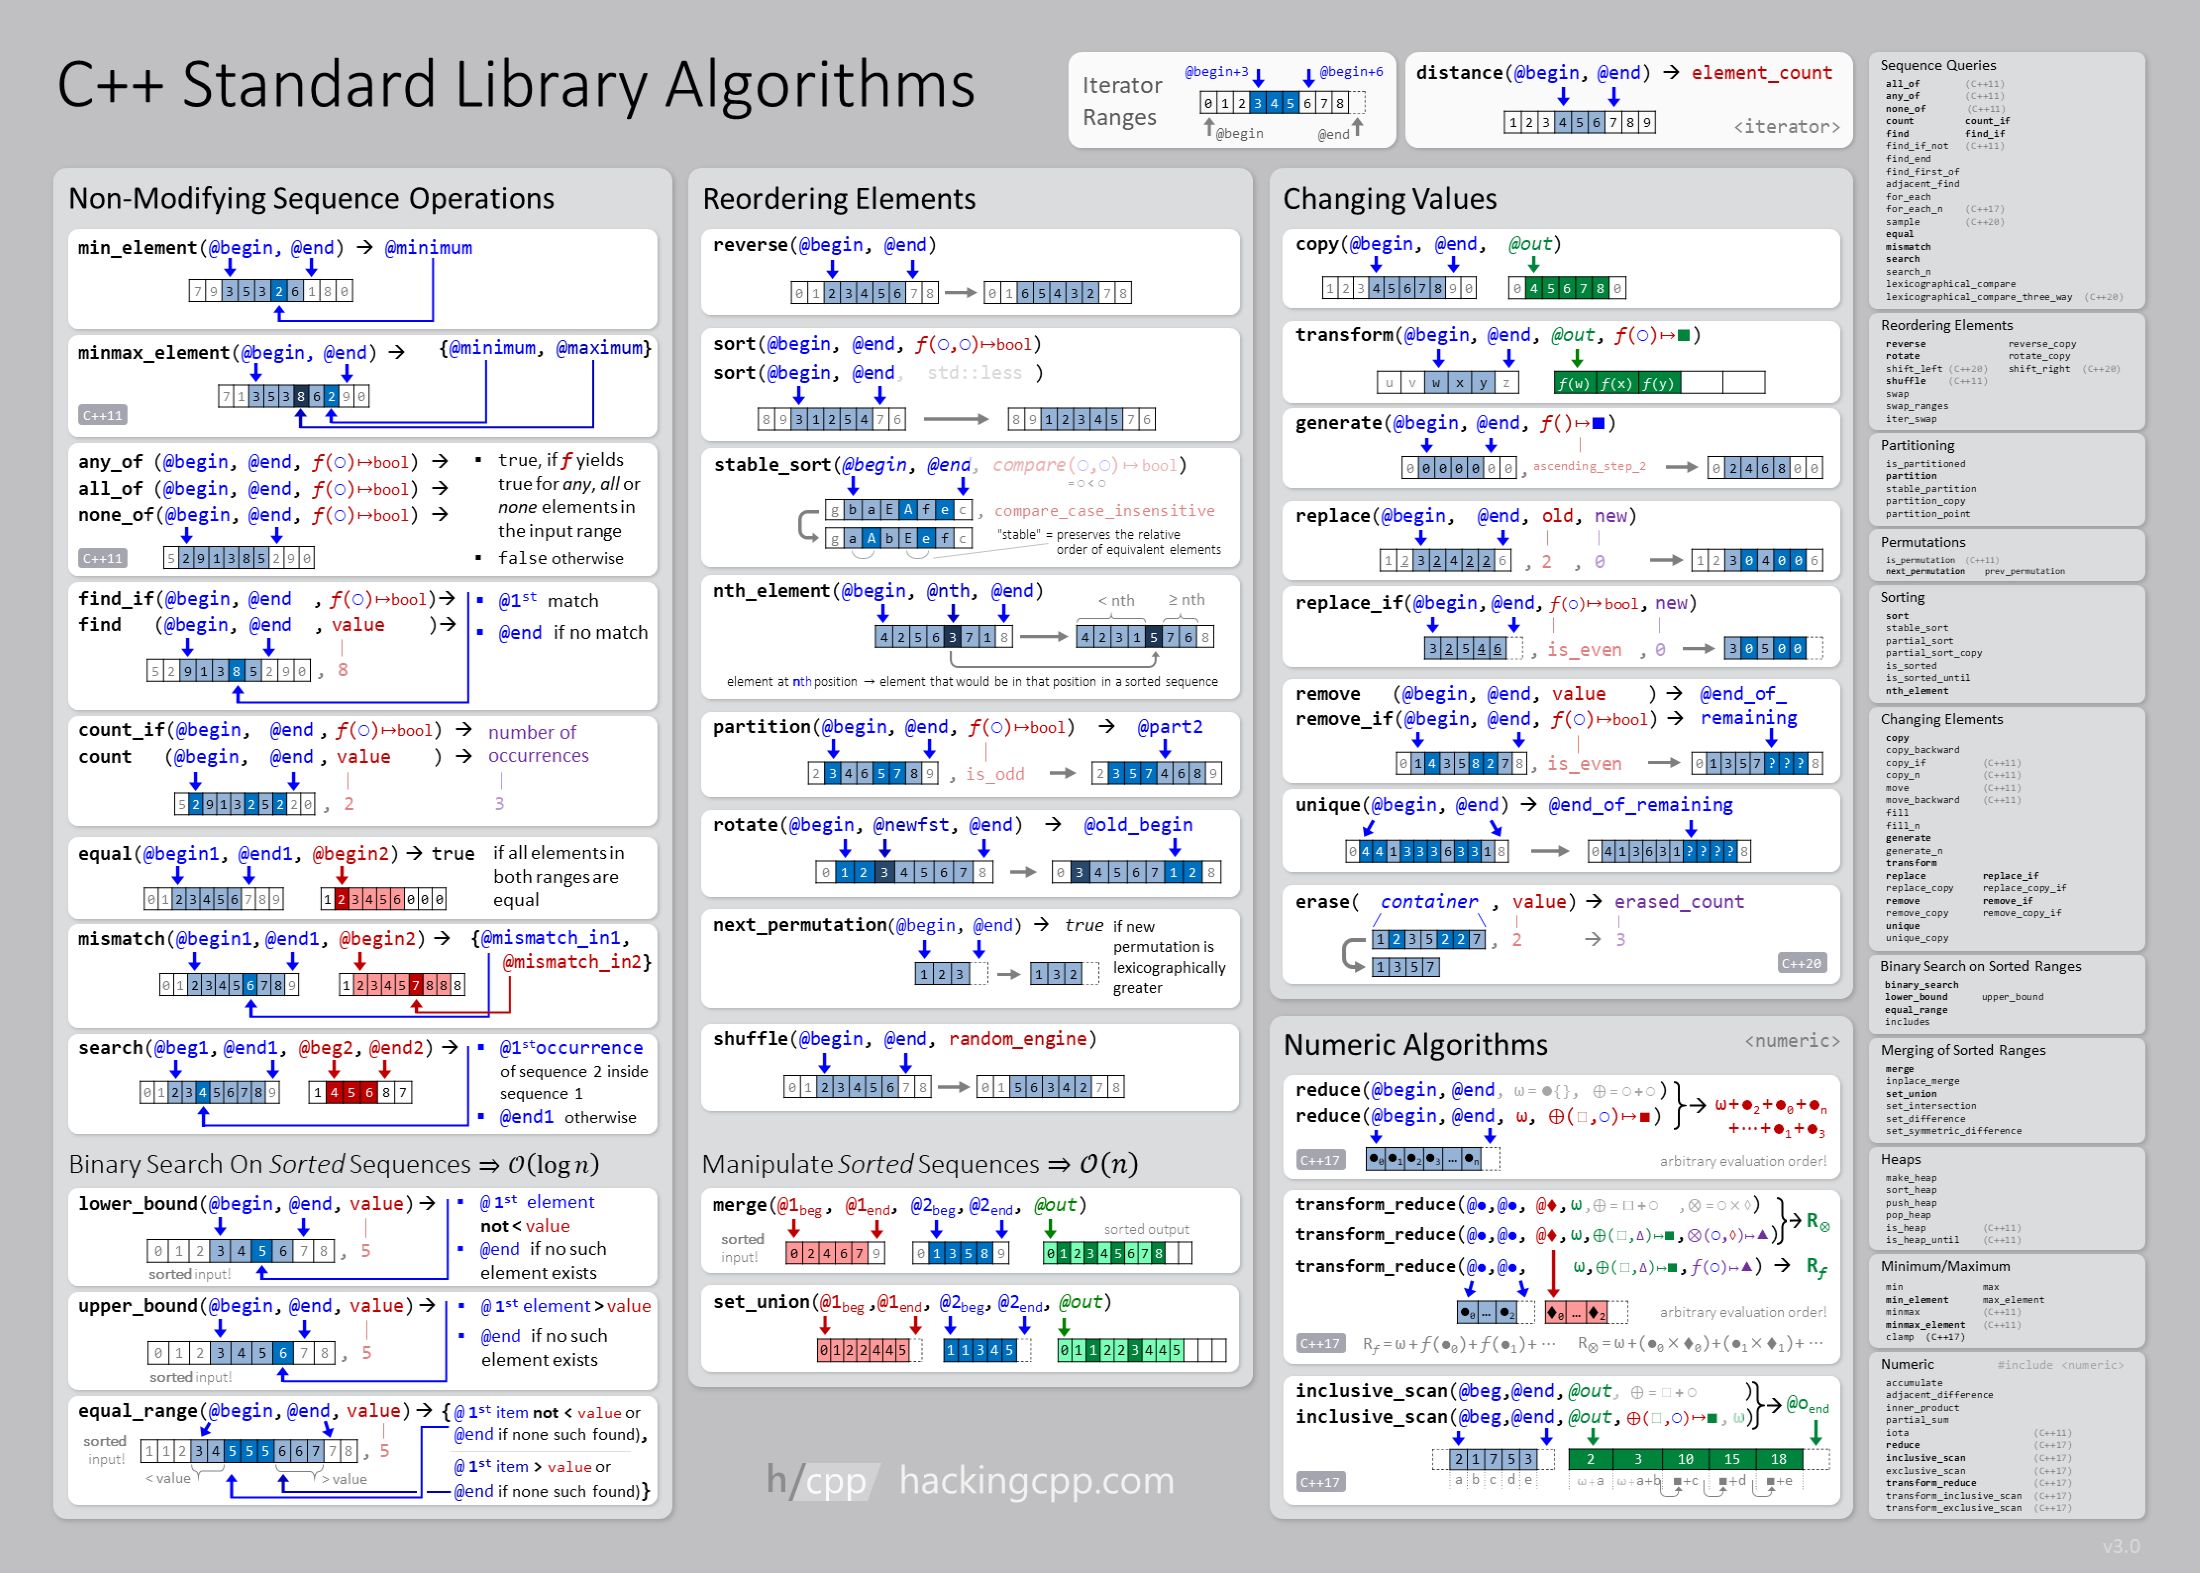
\includegraphics[width=1.2\textwidth, height=1.2\textheight, keepaspectratio]{./imgs/Algorithm_Library/algorithms.png}
	\caption{Algorithm Library}
	\label{fig:algorithms}
\end{figure}

%TODO: L'importanza della libreria degli algoritmi.
%TODO: Mettere in un itemize la lista di tutte le operazioni: operazioni su sequenze non modificabili, oprazioni su sequeunze modificabili, ecc... (magari in parantesi come è scritto in inglese)
%TODO: dire che non le tratterò proprio tutte tutte, alcune sono molto simili.

%TODO: Inoltre, dire che tratterò argomenti anche che non fanno parte della libreria degli Algoritmi, ma che possono essere utili da utilizzare assieme agli algoritmi.

% ------------------ SECTION: OPERAZIONI SU SEQUENZE NON-MODIFICABILI  ---------------

\newpage

\section{Operazioni su sequenze non-modificabili}

\textsf{\small \textbf{Definizione: } Le \textbf{operazioni su sequenze non-modificabili}, da come si intende sono quelle operazioni che non modificano la sequenza, ma che attuano, compiono ricerche per trovare determinati elementi, contano gli elementi, testano varie condizioni, eccetera..} \\

\subsection{Condizioni}

\textsf{\small Possiamo testare se degli elementi sono presenti o no attraverso queste funzioni: \textbf{std::all\_of}, \textbf{std::any\_of}, \textbf{std::none\_of}.} \\

\begin{itemize}
	\item \textsf{\small \textbf{any\_of} : ha bisogno che anche solo 1 sia vero (sia presente).}
	\item \textsf{\small \textbf{all\_of} : ha bisogno che tutti quelli considerati siano veri.}
	\item \textsf{\small \textbf{none\_of} : ha bisogno che nessuno sia presente (tra quelli cercati) (che siano tutti falsi).}
\end{itemize}

\begin{lstlisting}
	#include <iostream>
	#include <vector>
	#include <algorithm>
	
	int main()
	{
		std::vector<int> a = { 6, 1, 7, 3, 2, 5, 4, 9, 12 };
		std::vector<int> b = { 1, 4, 5, 8, 21, 11, 7, 0, 17 };
		
		// Ci assicuriamo che ci sia almeno un valore minore o uguale a 3 nel vettore a.
		std::cout << std::boolalpha << std::any_of( a.cbegin(), a.cend(), [](auto n) {return n <= 3; }) << "\n"; //Output: true
		
		// Ci assicuriamo che non ci siano valori maggiori di 33 nel vettore b.
		std::cout << std::boolalpha << std::none_of( b.cbegin(), b.cend(), [](auto n) { return n > 33; }) << "\n"; //Output: true
		
		std::vector<int> c = {0, 2, 4, 6, 8, 10};
		
		// Controlliamo se tutti i valori sono pari.
		if(std::all_of(c.cbegin(), c.cend(), [](int i){ return i % 2 == 0;}))
		{
			std::cout << "Tutti i numeri sono pari" << "\n";
		}
	
		//Output: Tutti i numeri sono pari.
		
		return 0;
	}	
\end{lstlisting}

\subsection{Ricerca}

\textsf{\small Queste operazioni servono per cercare degli elementi all'interno delle sequenze: \textbf{std::find}, \textbf{std::find\_if}, \textbf{std::find\_if\_not}, \textbf{find\_end}, \textbf{find\_first\_of}, \textbf{adjacent\_find}.} \\

\textsf{\small Inoltre ci sono anche: \textbf{std::search}, \textbf{search\_n}.} \\

\begin{lstlisting}
	#include <iostream>
	#include <string>
	#include <algorithm>
	#include <vector>
	
	int main()
	{
		// ESEMPIO FIND
		std::vector<std::string> a = { "zero", "one", "two", "three", "four", "five", "six", "seven", "eight", "nine", "ten" };
		std::vector<std::string> b = { "0", "1", "2", "3", "4", "5", "6", "7", "8", "9", "10" };
		
		// rbegin() e rend() servono per invertire (reverse) l'iteratore.
		const auto k = std::find( a.rbegin(), a.rend(), "one");
		std::cout << "Indice dell'ultimo 'one': " << (a.rend() - k) - 1 << std::endl; //Output: Indice dell'ultimo 'one': 1
		
		// ESEMPIO find\_first\_of
		const std::string s = "one;two,three:four";
		const std::string delimiter = ";,:";
		
		const auto i = std::find_first_of( s.cbegin(), s.cend(), delimiter.cbegin(), delimiter.cend());
		std::cout << "Indice del primo delimitatore: " << i - s.cbegin() << std::endl; //Output: Indice del primo delimitatore: 3
		
		// ESEMPIO adjacent\_find
		const std::string haystack = "as55jsdjflkadfkjsadlfs5j";
		const std::string needle = "s5j";
		
		const auto j = std::adjacent_find( haystack.cbegin(), haystack.cend() );
		std::cout << j - haystack.cbegin() << std::endl; //Output: 2
		
		// ESEMPIO SEARCH
		// Cerchiamo una sequenza nella stringa.
		const auto w = std::search( haystack.begin(), haystack.end(), needle.begin(), needle.end());
		std::cout << w - haystack.begin() << std::endl; //Output: 21
		return 0;
	}
\end{lstlisting}

\textsf{\small Questi sono alcuni esempi dell'utilizzo di questi funzioni, non li faccio tutti, ma gli altri sono intuitivi.} \\

\subsubsection{find vs search}

\textsf{\small La differenza è che \textbf{find} cerca un singolo elemento nella sequenza, mentre \textbf{search} cerca per un'intera sequenza nella sequenza. } \\

\subsection{Contatori}

\textsf{\small Ci sono un paio di funzioni per contare gli elementi di una sequenza: \textbf{std::count}, \textbf{std::count\_if}.} \\

\begin{lstlisting}
	#include <iostream>
	#include <algorithm>
	#include <vector>
	
	int main()
	{
		std::vector<int> v = { 8, 4, 9, 2, 3, 6, 5, 5, 1, 2, 4, 9, 1, 2};
		
		std::cout << std::count( v.begin(), v.end(), 3) << std::endl; //Output: 1
		
		std::cout << std::count_if( v.begin(), v.end(), [](auto n) { return n <= 7;}) << std::endl; //Output: 11
		return 0;
	}
\end{lstlisting}

\subsection{Altre operazioni}

\textsf{\small Ulteriori operazioni possibili sono: } \\

\begin{itemize}
	\item \textsf{\small \textbf{mismatch} : restituisce la prima posizione in cui due sequenze differiscono.}
	\item \textsf{\small \textbf{equal} : per controllare se due sequenze sono uguali (lo tratterò anche nelle \emph{Operazioni di Comparazione}).}
	\item \textsf{\small \textbf{is\_permutation} : testa se la sequenza è una permutazione (lo tratterò anche nelle \emph{Operazioni di Permutazione}).}
\end{itemize}

\begin{lstlisting}
	#include <iostream>
	#include <algorithm>
	#include <vector>
	
	int main()
	{
		// ESEMPIO MISMATCH
		std::vector<std::string> a = { "0", "1", "2", "3", "4", "5", "6", "7", "8", "9", "10" };
		std::vector<std::string> b = { "0", "1", "2", "3", "4", "&", "6", "7", "8", "9", "10" };
		
		const auto i = std::mismatch( a.cbegin(), a.cend(), b.cbegin()).first;
		std::cout << i - a.cbegin() << std::endl; //Output: 5
		
		// ESEMPIO EQUAL
		std::vector<int> v1 = { 1, 2, 3, 4, 5, 6 };
		std::vector<int> v2 = { 1, 2, 3, 4, 5, 6 };
		std::vector<int> v3 = { 1, 2, 4, 3, 5, 6 };
		
		std::cout << std::boolalpha << std::equal( v1.cbegin(), v1.cend(), v2.cbegin()) << std::endl; //Output: true
		std::cout << std::boolalpha << std::equal( v1.cbegin(), v1.cend(), v3.cbegin()) << std::endl; //Output: false
		
		// ESEMPIO IS\_PERMUTATION
		std::vector<int> vec = { 1, 2, 3, 4 };
		std::vector<int> vec2 = { 2, 3, 4, 1 };
		std::vector<int> vec3 = { 2, 3, 2, 2 };
		
		std::cout << std::boolalpha << std::is_permutation(vec.begin(), vec.end(), vec2.begin()) << std::endl; //Output: true
		std::cout << std::boolalpha << std::is_permutation(vec.begin(), vec.end(), vec3.begin()) << std::endl; //Output: false
		return 0;
	}
\end{lstlisting}

\fleuron %TODO: oppure \ornament

\textsf{\small Per tutte queste operazioni c'è un equivalente per \emph{ranges} del C++20 a pag. \pageref{ranges}} \\

% ------------------ SECTION: OPERAZIONI SU SEQUENZE MODIFICABILI --------------------

\newpage

\section{Operazioni su sequenze modificabili}

\textsf{\small \textbf{Definizione: } Queste, invece sono quelle operazioni che ti permettono di modificare la sequenza originaria.} \\

\subsection{Copiare sequenze}

\textsf{\small Queste operazioni ti permettono di copiare parti o intere sequenze: \textbf{std::copy}, \textbf{std::copy\_n}, \textbf{std::copy\_if}, \textbf{std::copy\_backward}.} \\

\begin{lstlisting}
	#include <iostream>
	#include <algorithm>
	#include <vector>
	#include <string>
	#include <iterator> // per usare gli iteratori nei loops.
	#include <cctype> // per usare std::isupper.
	
	int main()
	{
		// ESEMPIO COPY\_N
		std::vector<std::string> b = { "0", "1", "2", "3", "4", "5", "6", "7", "8", "9", "10" };
		
		std::vector<std::string> c;
		
		c.resize(9);
		
		std::copy_n( b.begin(), 9, c.begin());
		
		// A sto giro devo usare begin() ed end(), non posso usare cbegin() e cend().
		std::cout << "il vettore c contiene: ";
		for (std::vector<std::string>::iterator it = c.begin(); it!=c.end(); ++it)
		{
			std::cout << ' ' << *it;
		}
	
		std::cout << '\n';
	
		//Output: il vettore c contiene: 0 1 2 3 4 5 6 7 8
		
		// ESEMPIO COPY\_N 2
		std::string in = "1234567890";
		std::string out;
		
		std::copy_n(in.begin(), 4, std::back_inserter(out));
		std::cout << out << '\n'; //Output: 1234
		
		// ESEMPIO COPY\_IF
		std::string a = "Solo Le Lettere in Maiuscolo Verranno Considerate";
		
		std::string uppers;
		
		// back\_inserter è uno speciale tipo di \emph{output iterator} per 
		// permettere agli algoritmi che sovrascrivono gli elementi, come il 
		// \emph{copy} di inserire in dei nuovi elementi automaticamente alla fine del container.
		std::copy_if(a.begin(), a.end(), std::back_inserter( uppers ), [](auto s){ return std::isupper(s); } ); // una volta funzionava anche così: std::copy\_if(a.begin(), a.end(), std::back\_inserter( uppers), std::isupper);
		std::cout << uppers << std::endl; //Output: SLLMVC
		
		// ESEMPIO COPY\_BACKWARD
		std::vector<int> inVector;
		for(int i = 0; i < 10; i++)
		{
			inVector.push_back(i);
		}
	
		std::vector<int> outVector(15);
		
		std::copy_backward(inVector.begin(), inVector.end(), outVector.end());
		
		std::cout << "outVector contiene: ";
		for(auto v : outVector){
			std::cout << v << " ";
		}
	
		//Output: outVector contiene: 0 0 0 0 0 0 1 2 3 4 5 6 7 8 9
		return 0;
	}
\end{lstlisting}

\subsection{Move}

\textsf{\small Queste ci permettono di spostare gli elementi da una sequenza ad un'altra: \textbf{std::move}, \textbf{std::move\_backward}.} \\

\begin{lstlisting}
	#include <iostream>
	#include <vector>
	#include <string>
	#include <algorithm>
	
	int main()
	{
		std::vector<std::string> a = { "zero", "one", "two", "three", "four", "five", "six", "seven", "eight", "nine", "ten" };
		std::vector<std::string> b = { "0", "1", "2", "3", "4", "&", "6", "7", "8", "9", "10" };
		
		// Sposta i primi due parametri di move nell'inizio del suo terzo parametro.
		std::move( a.begin(), a.begin() + 3, b.begin()); // anche mettendo a.begin() funziona.
		
		std::cout << "il vettore a contiene: ";
		for(auto v : a){
			std::cout << v << " ";
		}
	
		//Output: Il vettore a contiene: three four five six seven eight nine ten
		
		return 0;
	}
\end{lstlisting}

\subsection{Swap}

\textsf{\small Le operazioni di \textbf{swap} ci permettono di scambiare gli elementi di due sequenze, contenitore: \textbf{std::swap}, \textbf{std::swap\_ranges}, \textbf{iter\_swap}.} \\

\begin{lstlisting}
	#include <iostream>
	#include <algorithm>
	#include <vector>
	
	int main()
	{
		// ESEMPIO SWAP
		int x = 5, int y = 12;
		
		std::cout << "x prima dello swap: " << x << ", y prima dello swap: " << y << std::endl; //Output: x prima dello swap: 5, y prima dello swap: 12
		
		std::swap(x,y);
		
		std::cout << "x dopo lo swap: " << x << ", y dopo lo swap: " << y << std::endl; //Output: x dopo lo swap: 12, y dopo lo swap: 5
		
		//ESEMPIO SWAP\_RANGES
		std::vector<int> vec1(7, 66);
		std::vector<int> vec2(7, 18);
		
		std::swap_ranges(vec1.begin() + 1, vec1.end() - 1, vec2.begin());
		
		std::cout << "vec1 contiene: ";
		for(auto v : vec1){
			std::cout << v << " ";
		}
	
		//Output: vec1 contiene: 66 18 18 18 18 18 66
		
		std::cout << '\n';
		
		std::cout << "vec2 contiene: ";
		for(auto v : vec2){
			std::cout << v << " ";
		}
	
		//Output: vec2 contiene: 66 66 66 66 66 18 18
		
		std::cout << '\n';
		return 0;
	}
\end{lstlisting}

\subsection{Transform}

\textsf{\small Applica un'operazione sugli elementi delle sequenze: \textbf{std::transform}.} \\

\textsf{\small \textbf{In Place} : vuol dire che il risultato viene messo nello stesso contenitore non in un altro a parte.} \\

\begin{lstlisting}
	#include <iostream>
	#include <algorithm>
	#include <vector>
	#include <cctype>
	
	int main()
	{
		// ESEMPIO 1
		std::vector<int> a = { 5, 7, 8, 9, 1, 2};
		std::vector<int> b = { 3, 6, 2, 1, 0, 9};
		
		std::vector<int> c;
		
		std::transform( a.begin(), a.end(), b.begin(), std::back_inserter(c), [](int a, int b) { return a + b * b; });
		
		std::cout << "c contiene: ";
		for(auto v : c)
		{
			std::cout << v << " ";
		}
		
		std::cout << '\n';
		
		//Output: c contiene: 14 43 12 10 1 83
		
		//ESEMPIO 2
		std::string s = "Questa frase verra\' trasformata";
		std::string out;
		
		std::transform( s.begin(), s.end(), std::back_inserter(out), [](auto o){return std::toupper(o);});
		
		std::cout << out << '\n';
		
		//Output: QUESTA FRASE VERRA' TRASFORMATA
		return 0;
	}
\end{lstlisting}

\subsection{Replace}

\textsf{\small Queste permettono di rimpiazzare alcuni elementi della sequenza con altri: \textbf{std::replace}, \textbf{std::replace\_if}, \textbf{std::replace\_copy}, \textbf{std::replace\_copy\_if}.} \\

\begin{lstlisting}
	#include <iostream>
	#include <algorithm>
	#include <vector>
	
	int main()
	{
		return 0;
	}
\end{lstlisting}

\begin{comment}
\begin{lstlisting}
	#include <iostream>
	#include <algorithm>
	#include <vector>
	
	int main()
	{
		return 0;
	}
\end{lstlisting}
\end{comment}

% ---------------------- SECTION: OPERAZIONI SU PARTIZIONI ---------------------------

% --------------------- SECTION: OPERAZIONI DI ORDINAMENTO ---------------------------

% ------------ SECTION: OPERAZIONI DI RICERCA BINARIA (BINARY SEARCH) ----------------

% --------------- SECTION: ALTRE OPERAZIONI DI ORDINAMENTO SUI RANGES ----------------

%TODO: questa parte nella sezione sul C++20

% ------------------------ SECTION: OPERAZIONI SUGLI INSIEMI -------------------------

% ------------------------- SECTION: OPERAZIONI SU HEAP ------------------------------

% ------------------------- SECTION: OPERAZIONI DI MIN/MAX ---------------------------

% ----------------------- SECTION: OPERAZIONI DI COMPARAZIONE ------------------------

% ---------------------- SECTION: OPERAZIONI SU PERMUTAZIONI -------------------------

% -------------------------- SECTION: OPERAZIONI NUMERICHE ---------------------------

% ------------------ SECTION: OPERAZIONI SU MEMORIA INIZIALIZZATA --------------------

% ------------------------------ SECTION: OPTIONALS ----------------------------------

%TODO: optionals in default parameters in functions.

% ------------------------- SECTION: EXECUTION POLICIES ------------------------------

% -------------------------------- SECTION: C++20 ------------------------------------

\label{ranges}

%TODO: La roba del C++20 come ultimo argomento del capitolo.
%TODO: ranges, concepts, constrained algorithms, coroutines, template parameter list, modules, ecc..
%TODO: non tutte queste c'entrano con la libreria degli algoritmi, le altre le potrei trattare nel capitolo 'Concetti Avanzati' (visto che è anche il più corto)
%TODO: tipo la libreria <coroutine>, <concepts>, ecc..

% ------------------------------ FINE CAPITOLO ---------------------------------------